\chapter*{Appendix}

\begin{figure}[t]
    \centering
        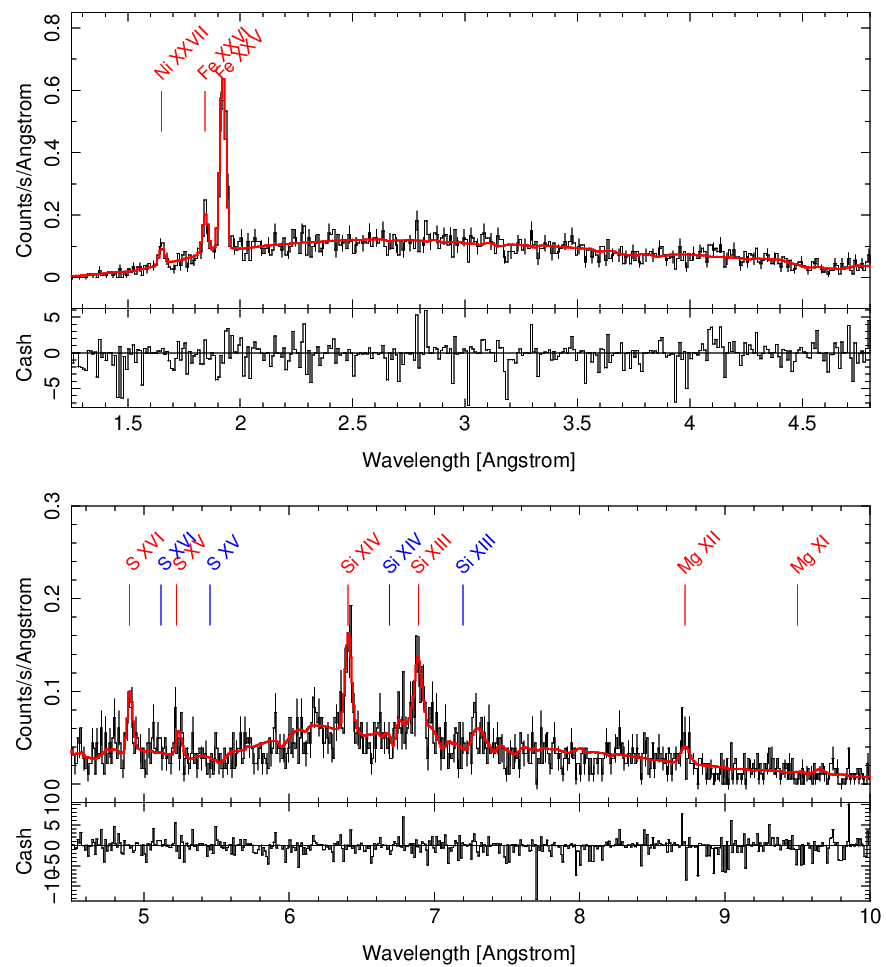
\includegraphics[width = \linewidth]{Chapters/Figures/long_pheno0_heg.png}
        \caption{The X-ray spectrum of SS 433 observed with the Chandra HETGS on 2018-08-13, when the accretor's orbit phase is 0.022. This set of figures show the spectrum formed from the HEG data of the first 19.2 ksec of the long observation. The disappearance of Fe {\sc xxv} indicates that the region of the Eastern jet showing Fe {\sc xxv} is blocked.}
    \label{long_pheno0_heg}
\end{figure}


\begin{figure}[t]
    \centering
        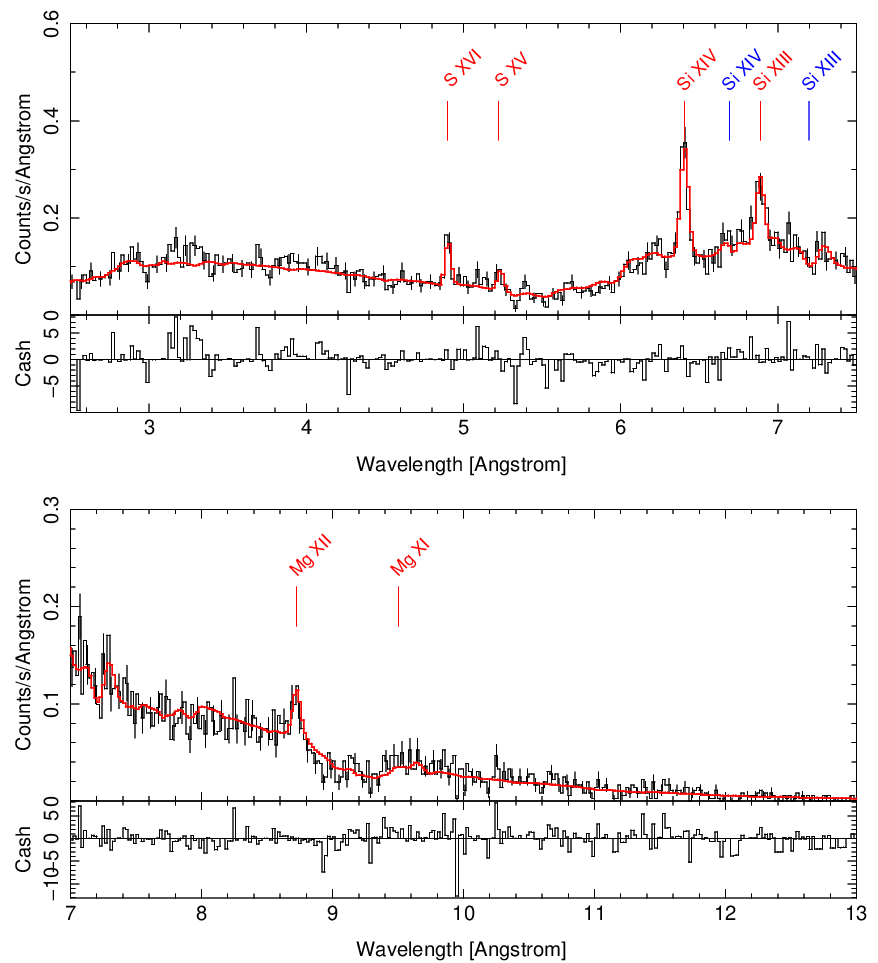
\includegraphics[width = \linewidth]{Chapters/Figures/long_pheno0_meg.png}
        \caption{Same as Figure~\ref{long_pheno0_heg}, but showing the MEG spectrum.}
    \label{long_pheno0_meg}
\end{figure}





\begin{figure}[t]
    \centering
        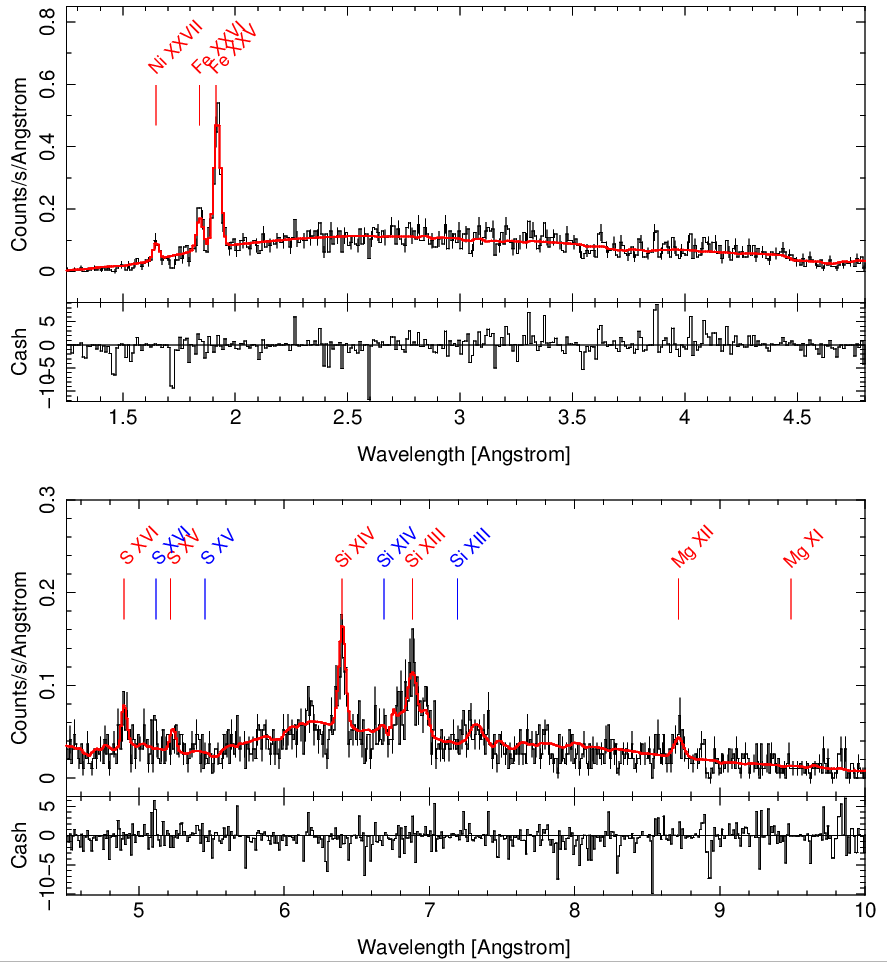
\includegraphics[width = \linewidth]{Chapters/Figures/long_pheno1_heg.png}
        \caption{Same as Figure~\ref{long_pheno0_heg} but showing the spectrum from the HEG data of the second 19.2 ksec of the long observation. The orbit phase of the accretor is 0.039.}
    \label{long_pheno1_heg}
\end{figure}


\begin{figure}[t]
    \centering
        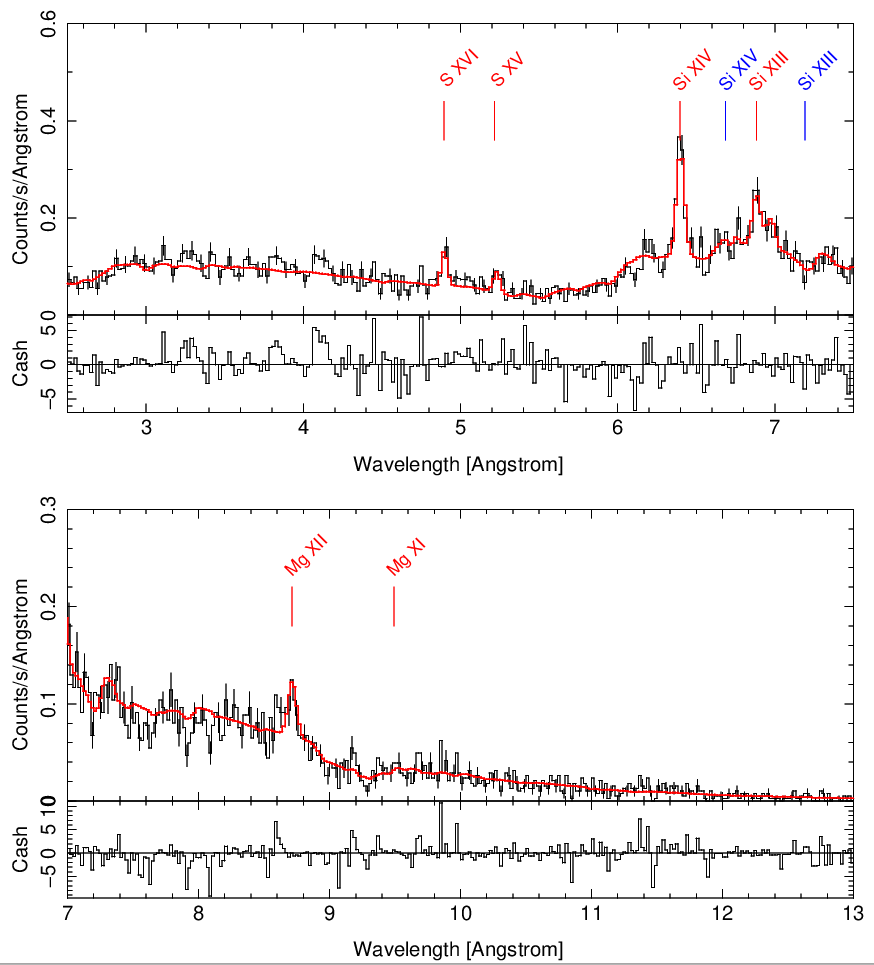
\includegraphics[width = \linewidth]{Chapters/Figures/long_pheno1_meg.png}
        \caption{Same as Figure~\ref{long_pheno1_heg}, but showing the MEG spectrum.}
    \label{long_pheno1_meg}
\end{figure}


\begin{figure}[t]
    \centering
        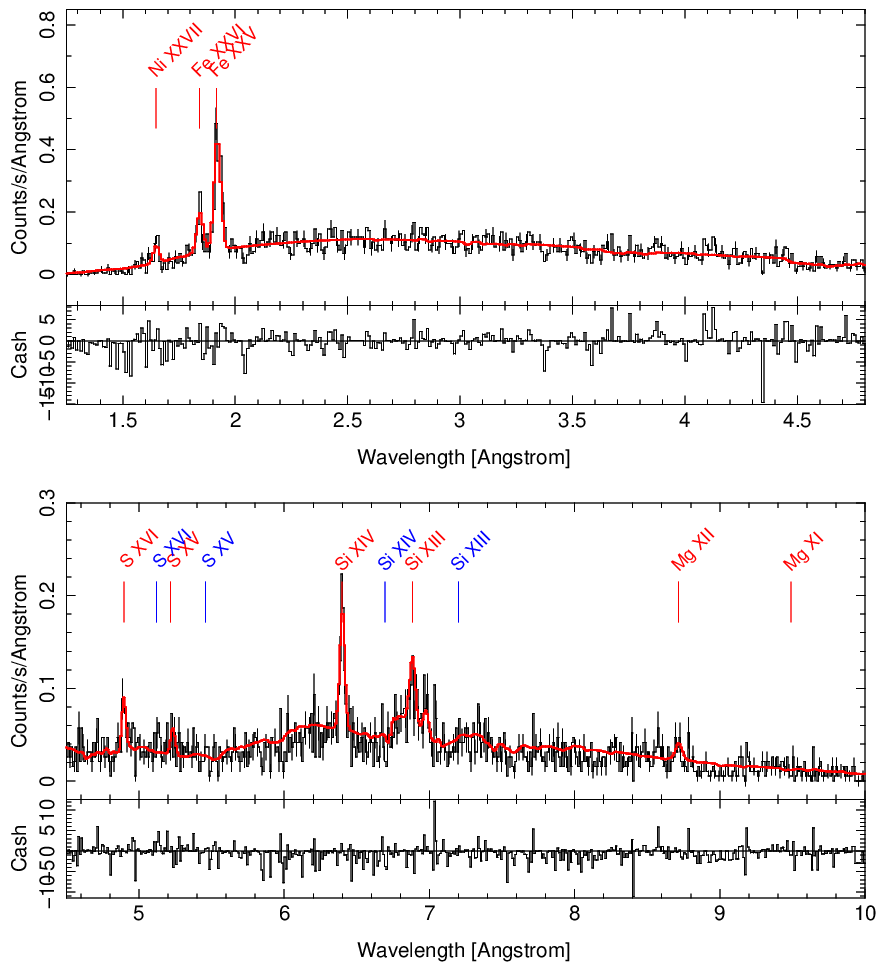
\includegraphics[width = \linewidth]{Chapters/Figures/long_pheno2_heg.png}
        \caption{Same as Figure~\ref{long_pheno0_heg} but showing the spectrum formed from the HEG data of the third 19.2 ksec part of the long observation. The orbit phase of the accretor is 0.057.}
    \label{long_pheno2_heg}
\end{figure}


\begin{figure}[t]
    \centering
        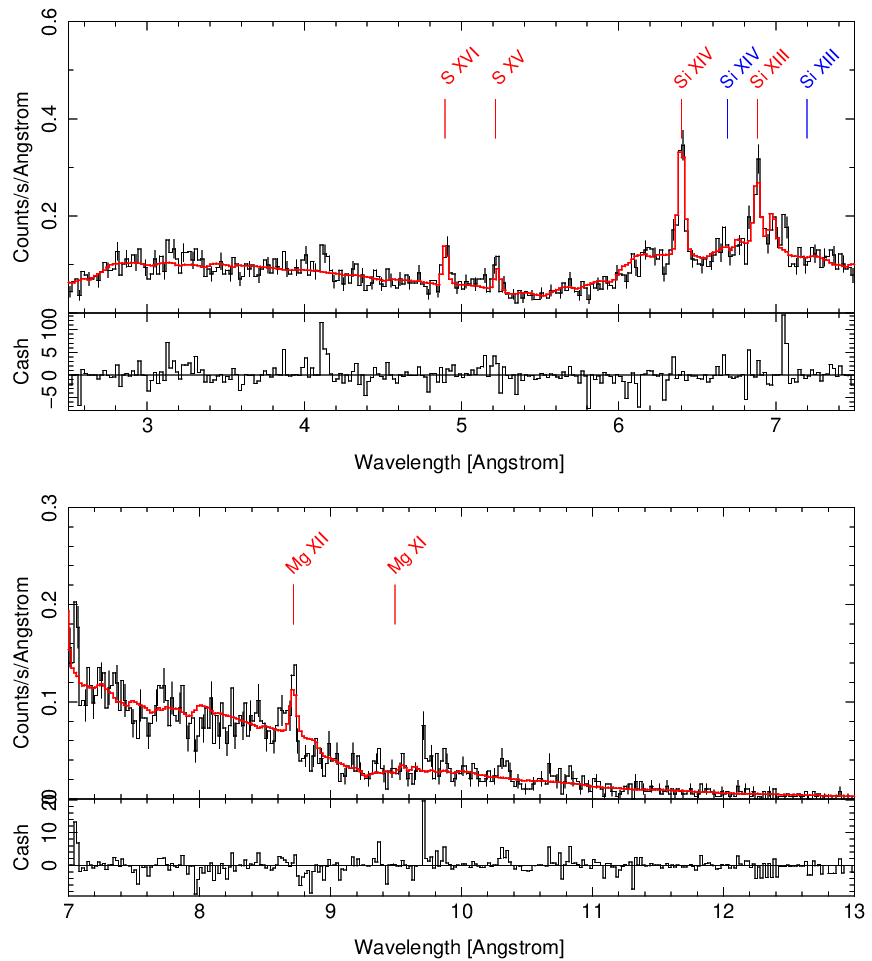
\includegraphics[width = \linewidth]{Chapters/Figures/long_pheno2_meg.png}
        \caption{Same as Figure~\ref{long_pheno2_heg}, but showing the MEG spectrum.}
    \label{long_pheno2_meg}
\end{figure}


\begin{figure}[t]
    \centering
        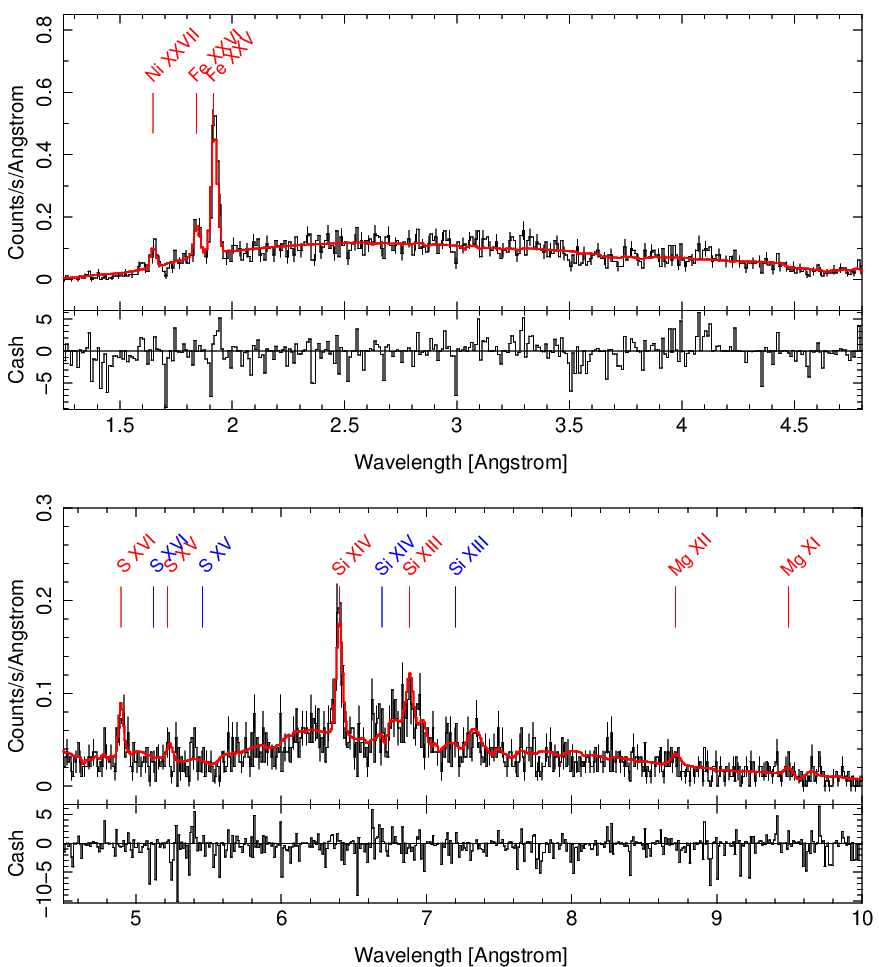
\includegraphics[width = \linewidth]{Chapters/Figures/long_pheno3_heg.png}
        \caption{Same as Figure~\ref{long_pheno0_heg} but showing the spectrum formed from the HEG data of the fourth 19.2 ksec of the long observation. The orbit phase of the accretor is 0.074.}
    \label{long_pheno3_heg}
\end{figure}


\begin{figure}[t]
    \centering
        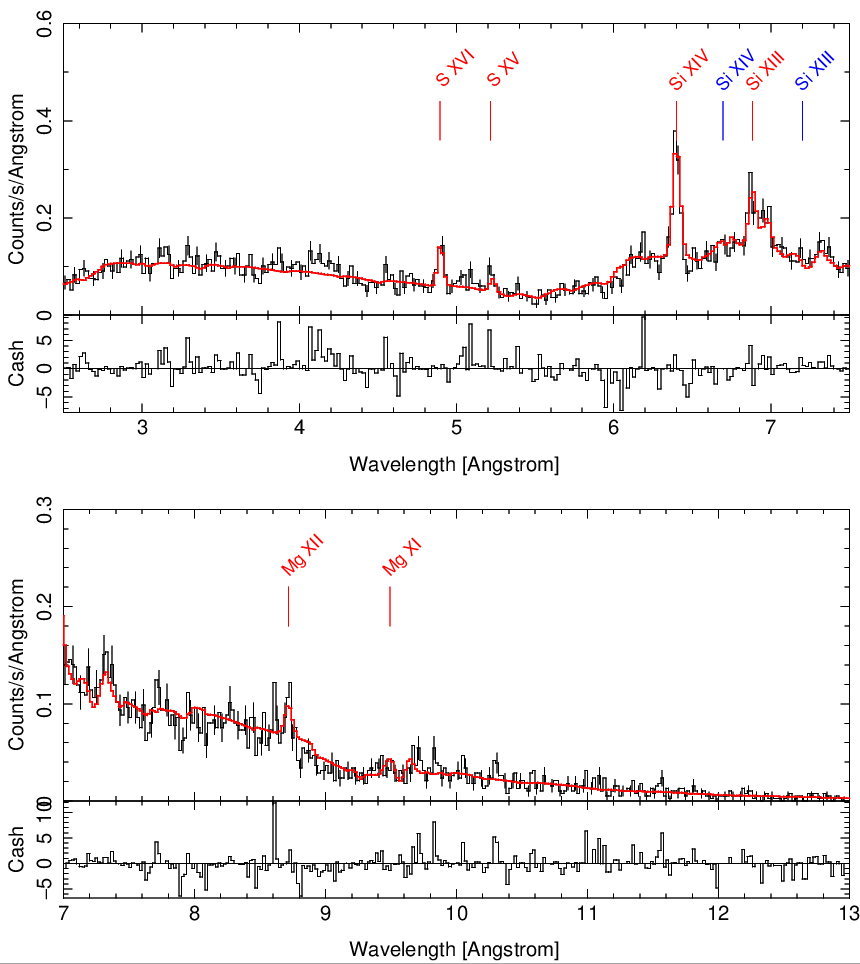
\includegraphics[width = \linewidth]{Chapters/Figures/long_pheno3_meg.png}
        \caption{Same as Figure~\ref{long_pheno3_heg}, but showing the MEG spectrum.}
    \label{long_pheno3_meg}
\end{figure}



\begin{figure}[t]
    \centering
        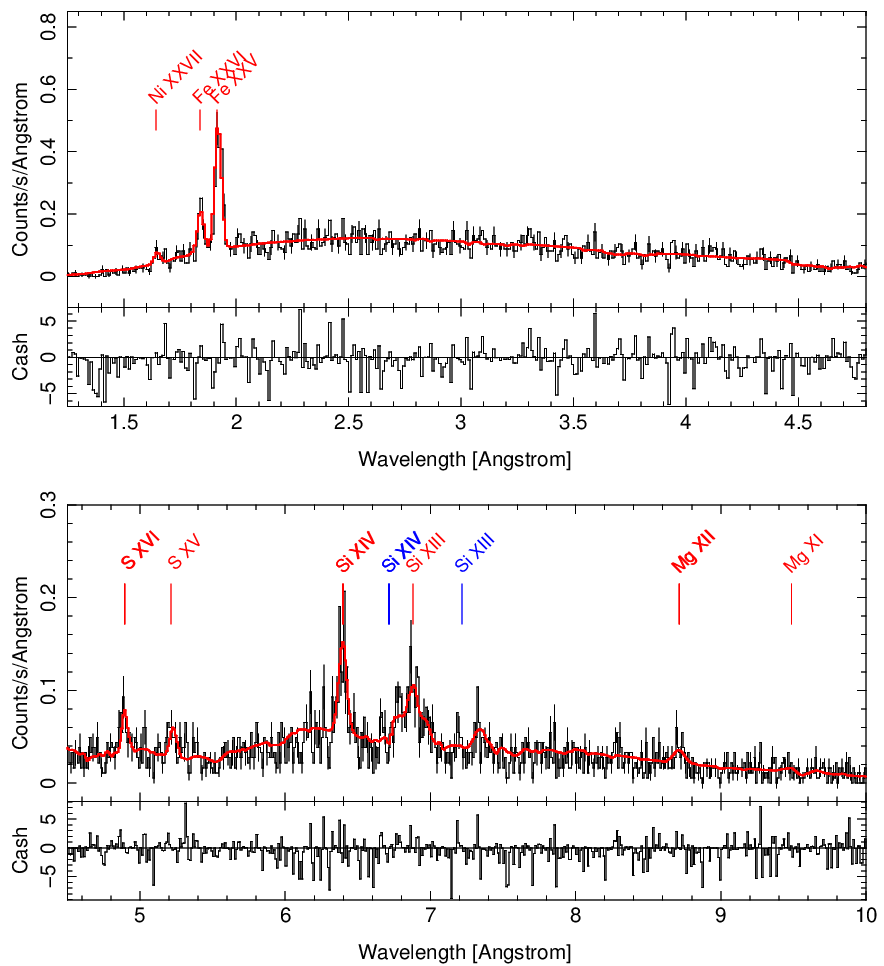
\includegraphics[width = \linewidth]{Chapters/Figures/long_pheno4_heg.png}
        \caption{Same as Figure~\ref{long_pheno0_heg} except this set of figures show the spectrum formed from the HEG data of the fifth 19.2 ksec of the long observation. The orbit phase of the accretor is 0.092. It is noticeable that the Fe {\sc xxv} from the Eastern jet did not reappear in the spectra as predicted by the ephemeris.}
    \label{long_pheno4_heg}
\end{figure}


\begin{figure}[t]
    \centering
        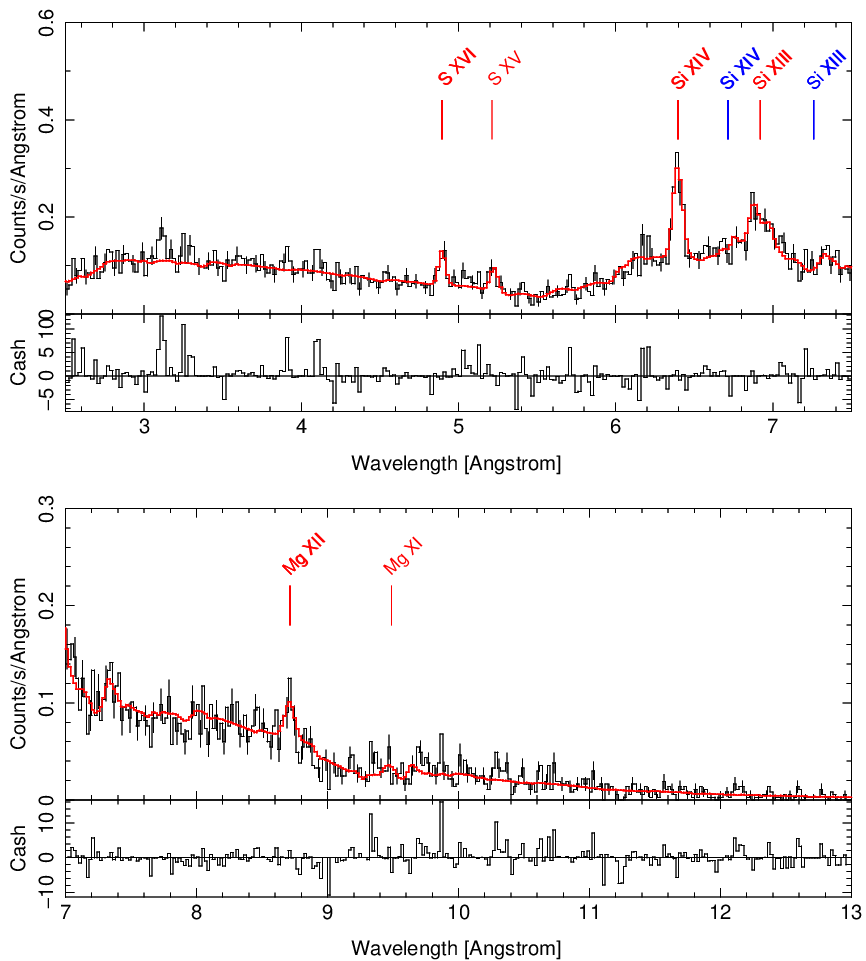
\includegraphics[width = \linewidth]{Chapters/Figures/long_pheno4_meg.png}
        \caption{Same as Figure~\ref{long_pheno4_heg}, but showing the MEG spectrum}
    \label{long_pheno4_meg}
\end{figure}